\clearpage

\section {Neutrino oscillation fitting}
\label{sec:oscfit}

%--------------------------------------------------------------------------------------------------------------------
\subsection {Fit method}
\label{sec:oscfit_method}

Several choices exist for the 23-sector oscillation parameters that could be fitted, 
and these choices have been presented in the context of the {\em VALOR} joint 3-flavour fit of the 1 $\mu$-like ring 
and 1 e-like ring reconstructed SuperK spectra \cite{Lorena}.
During the review process of the T2K Run 1+2+3 $\nu_{\mu}$-disappearance PRL \cite{T2KRun123Disapp}, it was discovered that the
choice of octant ($\theta_{23} \leq \pi/4$ or $\theta_{23} \geq \pi/4$) has a large effect on the confidence contour in $\sin^2(2\theta_{23})$.
Therefore, we now fit $\sin^2\theta_{23}$ by default. This is a sensible choice since the value of $\sin^2\theta_{23}$ giving
 maximal disappearance is not the same as the value giving maximal mixing ($\sin^2\theta_{23}$ = 0.5); this difference is 
due to the non-zero value of $\theta_{13}$.
There are also different choices for the mass-squared splitting parameter: typically $|\Delta m^{2}_{32}|$ is used in $\nu_{\mu}$-disappearance 
analyses, but this is the largest mass-squared splitting for the inverted mass
hierarchy and the second largest for the normal mass hierarchy. 
It is therefore not correct to compare results obtained under the different mass hierarchy hypotheses.
Other choices include fitting a mass-squared difference whose absolute value is the same for both mass hierarchies,
such as $\Delta m^{2} = \left(m_{3}^{2} - \frac {m_{1}^{2}+m_{2}^{2}} {2} \right)$ \cite{FogliLisi},
or fitting $|\Delta m^{2}_{32}|$ for one hierarchy and $|\Delta m^{2}_{31}|$ for the other \cite{GonzalezGarcia}.
All these choices are implemented in the {\em VALOR} oscillation analysis framework, and our analysis can switch between them.
For the present analysis, it was decided to fit 
$|\Delta m^{2}_{32}|$ for the normal hierarchy and $|\Delta m^{2}_{31}|$ for the inverted hierarchy. The actual inputs to the calculation 
of the oscillation probabilities are +$|\Delta m^{2}_{32}|$ for the normal hierarchy and -$|\Delta m^{2}_{31}|$ for the inverted hierarchy.
Fits of $|\Delta m^{2}_{32}|$ for the inverted hierarchy were also performed for validation.

The {\em VALOR} disappearance analysis uses a binned likelihood-ratio method.
Measurements of the oscillation parameters $\sin^{2}\theta_{23}$ and $|\Delta m^{2}_{32}|$ or $|\Delta m^{2}_{31}|$
are obtained by comparing the observed and predicted SuperK reconstructed energy spectra
for 1-ring $\mu$-like events.

Let $N$ be the number of reconstructed energy bins and
${\bf a}$ be a $1 \times N_{s}$ - dimensional array of systematic (nuisance) 
parameters that affect the SuperK reconstructed energy spectrum prediction (e.g
parameters that control the beam, neutrino interaction simulations and 
the detector response).
Best-fit values are obtained by minimizing: 
\begin{equation}
\displaystyle
%\chi^{2} 
-2 \; \textrm{ln} \; \lambda (\sin^{2}\theta_{23},|\Delta m^{2}_{32}| \; \textrm{or} \; |\Delta m^{2}_{31}|; {\bf a}) = 
  2 \cdot \sum_{i=0}^{N-1} 
   \Big( 
     n^{obs}_{i} \cdot ln(n^{obs}_{i}/n^{exp}_{i}) +
     (n^{exp}_{i}-n^{obs}_{i}) 
   \Big) +
   ({\bf a}-{\bf a_{0}})^{T} \cdot {\bf C}^{-1} \cdot ({\bf a}-{\bf a_{0}})
\label{eq:chisquare}
\end{equation}
where
${\bf a_{0}}$ is an $1 \times N_{s}$ - dimensional array with the default values of 
the systematics parameters, ${\bf a}^{T}$ is the transpose of ${\bf a}$,
${\bf C}$ is the systematic parameter covariance matrix of dimension $N_{s} \times N_{s}$,
$n^{obs}_{i}$ is the observed number of events in the $i^{th}$ bin, and
$n^{exp}_{i} = n^{exp}_{i}(\sin^{2}\theta_{23},|\Delta m^{2}_{32}| \; \textrm{or} \; |\Delta m^{2}_{31}|; {\bf a})$ 
is the corresponding expected number of events.

The likelihood-ratio method used in this analysis is equivalent to the extended maximum likelihood
method used in the alternative T2K oscillation analysis 
(see \cite{OurRun1DisappAnalysis,StatAnalysisCowan} for more details).
The advantage of the likelihood ratio method, compared with the extended maximum-likelihood method, is that
in the large-sample limit, the quantity $-2 \: \textrm{ln} \: \lambda (\sin^{2}\theta_{23},|\Delta m^{2}_{32}| \; \textrm{or} \; |\Delta m^{2}_{31}|; {\bf a})$
in Eq.\ref{eq:chisquare} has a $\chi^{2}$ distribution and it can therefore be used as a goodness-of-fit test.
In this note,
$-2 \: \textrm{ln} \: \lambda (\sin^{2}\theta_{23},|\Delta m^{2}_{32}| \; \textrm{or} \; |\Delta m^{2}_{31}|; {\bf a})$ and
$\chi^{2}(\sin^{2}\theta_{23},|\Delta m^{2}_{32}| \; \textrm{or} \; |\Delta m^{2}_{31}|; {\bf a})$ are used interchangeably.

The minimization is performed with Minuit \cite{Minuit}, using the Migrad method.
If Migrad does not converge, the starting values of the oscillation parameters are re-initialised:
the new initial values are randomly drawn from uniform distributions in the ranges 
$1.5 \times 10^{-3}$ eV$^{2}$/c$^{4}$ $\leq$ $|\Delta m^{2}_{32}| \; \textrm{or} \; |\Delta m^{2}_{31}|$ $\leq$ $3.5 \times 10^{-3}$  eV$^{2}$/c$^{4}$ and
either 0.35 $\leq$ $\sin^{2}\theta_{23}$ $\leq$ 0.50 or 0.53 $\leq$ $\sin^{2}\theta_{23}$ $\leq$ 0.68 (the new initial value of 
$\sin^{2}\theta_{23}$ is in the same octant as the previous initial value).  
The fit is retried with the new initial values, and this is repeated up to 10 times.
If the fit still fails to converge after 10 attempts, the Simplex algorithm is used.
The search for the minimum value of 
$-2 \: \textrm{ln} \: \lambda(\sin^{2}\theta_{23},|\Delta m^ {2}_{32}| \; \textrm{or} \; |\Delta m^{2}_{31}|; {\bf a})$ (see Eq. \ref{eq:chisquare}) 
is performed in the range 
$0 \leq$ $\sin^{2}\theta_{23}$ $\leq 1$ and
$1 \times 10^{-3}$ eV$^{2}$/c$^{4}$ $\leq$ $|\Delta m^{2}_{32}| \; \textrm{or} \; |\Delta m^{2}_{31}$ $\leq 6 \times 10^{-3}$ eV$^{2}$/c$^{4}$.
After a successful fit, The Hesse algorithm is called to improve Minuit's estimates of the
errors on the fitted parameters.

Each fit is repeated twice: in the first fit, the initial values are $|\Delta m^{2}_{32}|$ or $|\Delta m^{2}_{31}|$ = 2.4 $\times$ 10$^{-3}$ 
eV$^{2}$/c$^{4}$ and $\sin^{2}\theta_{23} = 0.6$, while the second fit uses as initial values the best fit of $|\Delta m^{2}_{32}|$ or $|\Delta m^{2}_{31}|$ 
and the mirror point in the other octant of the best fit of $\sin^{2}\theta_{23}$ from the first fit. 

All the systematic parameters are allowed to float in the fit, and are restricted to the range [-5$\sigma_{s}$, +5$\sigma_{s}$]
where $\sigma_{s}$ is the one standard deviation error assigned to each systematic parameter\footnote{
 Such an error is defined for all but one of the systematic parameters considered in this analysis. 
 The exception is the systematic parameters $f_{SF}$ which parameterizes the uncertainty on nuclear modelling,
 switching between the Relativistic Fermi Gas (RFG) and Spectral Function (SF) models. The allowed range of the parameter $f_{SF}$ 
 in the oscillation fit is [0,1].}.
Values of systematic parameters that give a negative predicted number of events in any reconstructed energy bin are not allowed. 
If this scenario arises, the number of events is changed to +1E-8 in that bin. This is done for the sum of all the interaction 
modes rather than for each mode separately.

In a 3-flavour $\nu_{\mu}$-disappearance fit, it is also necessary to make a choice for the treatment of the 
non-23-sector oscillation parameters. In the current analysis, we allow each of
$\sin^{2}(2 \theta_{13})$, $\sin^{2}(2 \theta_{12})$, $\Delta m_{21}^{2}$ and $\delta_{CP}$ to float. 
We use penalty terms for $\sin^{2}(2 \theta_{13})$, $\sin^{2}(2 \theta_{12})$, $\Delta m_{21}^{2}$, and their central values 
and uncertainties are shown in Tab.\ \ref{tab:pdg2012non23}; these are taken from the 2012 PDG \cite{PDG2012}\footnote{
  Note that in
  parts of Sec.\ \ref{sec:systematics:evaluation} (Figs.\ \ref{fig:1Rmu_error_ratio_to_nominal_osc}-\ref{fig:1Rmu_systematics_spread_by_group_osc}
  and Tabs.\ \ref{tab:star_summary_by_mixing}-\ref{tab:star_summary_by_mass}),
  Sec.\ \ref{sec:validation},
  and parts of Sec.\ \ref{sec:results} (critical $\Delta\chi^2$ calculatations and Fig.\ \ref{fig:results_compare_constdchisq_sensitivity_normal}),
  a value for $\sin^{2}(\theta_{12})$ of 0.306 with 1$\sigma$ range of 5.9\% \cite{FogliLisi} is used.
  The data best-fit point, 1D limits, and contours are identical using this number.
}.
There is no penalty term for 
$\delta_{CP}$, and it is allowed to float freely in the range [$-\pi$, $+\pi$]\footnote{
 The \emph{non-23-sector} oscillation parameters are allowed to float in the fit in the following ranges:
 $\sin^{2}\theta_{12}$ and $\sin^{2}\theta_{13}$ in the range [0,1];
 $\Delta m^{2}_{21}$ in the range [6,9] $\times 10^{-3} eV^{2}/c^{4}$;
 and $\delta_{CP}$ in the range [$-\pi$, $+\pi$].
}.
\begin{table}
\centering
\begin{tabular}{| c | c | c | }
\hline
Parameter                  &  Best-fit                                    & 1$\sigma$ range  \\
\hline
$\Delta m_{21}^{2}$        &  7.5 $\times$ 10$^{-5}$ eV$^{2}$/c$^{4}$     & $\pm\sim$2.7\% \\
$\sin^{2}(\theta_{12})$    &  0.312                                       & $\pm\sim$5.8\% \\
$\sin^{2}(\theta_{13})$    &  0.0251                                      & $\pm\sim$13.9\% \\
%$\delta_{CP}$              &  -                                           & [-$\pi$,+$\pi$] \\
\hline
\end{tabular}
\caption{
  Best-fit values and 1$\sigma$ range for the measured \emph{non-23-sector} oscillation parameters \cite{PDG2012}.
  $\delta_{CP}$ is allowed to float freely in the range [$-\pi$, $+\pi$] without penalty.
}
\label{tab:pdg2012non23}
\end{table}

%--------------------------------------------------------------------------------------------------------------------

\subsection {Goodness-of-fit tests}
\label{sec:gof_test}

In our $\nu_{\mu}$-disappearance analysis of the Run1+2 datasets, p-values were computed using both 
a) the rate of single $\mu$-like ring events and 
b) the rate and reconstructed energy distribution of single $\mu$-like ring events using the likelihood-ratio method \cite{NickPvalue}.
The choice is not unique.

D. Karlen has pointed out that, if the statistics are low, ``the use of the
distribution is not helpful in forming the p-value. 
This is directly related to the well known problem that is difficult to define
a general goodness-of-fit for sparsely populated distributions.
Large bins (or in the extreme a single bin = rate-only)
are necessary for small statistics samples'' \cite{KarlenPvalue}.

It was decided by the oscillation analysis group that, for all $\nu_{\mu}$-disappearance analyses, 
p-values will be calculated using the rate and the reconstructed energy distribution,
and that the distribution will use a very coarse binning
scheme to ensure that there are sufficient numbers of events in each bin: 
this scheme has 5 bins from 0-0.4, 0.4-0.7, 0.7-1.0, 1.0-2.0 and 2.0-30.0 GeV.

%--------------------------------------------------------------------------------------------------------------------
\subsection {Construction of confidence regions}
\label{sec:contour_construction}

In this analysis, uncertainties in the jointly measured parameters are quoted using both 
the constant-$\Delta\chi^{2}$ \cite{PDG2012} (pp. 390-401)
and the Feldman-Cousins \cite{FeldmanCousins} methods.
A definite recommendation was made in favour of the Feldman and Cousins method 
for constructing confidence regions by the T2K $\nu_{\mu}$ contour committee \cite{T2KNuMuContourCom}.
The work of Feldman and Cousins 
uses the freedom which is inherent in the Neyman construction of confidence regions
to address cases 
(in particular, cases with
Poisson processes with background and Gaussian errors near a physical boundary)
where the classical construction of confidence regions produces overcoverage, undercoverage, or
in extreme cases, an empty region.

The two methods have been described in detail in past T2K technical notes and presentations.
For completeness, we summarise both of these methods here
and provide definite statements on the exact methodology used for incorporating systematic errors.

The methods differ in the calculation of the critical values of $\Delta{\chi^{2}}$, which are used to identify the areas 
of the parameter space to be included in the allowed region for a given confidence level. The constant-$\Delta\chi^{2}$ 
method is a fully frequentist treatment using the Gaussian approximation.
One finds the best-fit point and calculates the confidence contours as lines of \emph{constant} $\Delta{\chi^{2}}$
from this point\footnote{
For 1 fit parameter, the critical values of $\Delta{\chi^{2}}$ used are
1.00 (68\% CL), 2.71 (90\% CL), 3.84 (95\% CL), 6.63 (99\% CL).
For 2 parameters fitted simultaneously, the critical values of $\Delta{\chi^{2}}$ used are
2.30 (68\% CL), 4.61 (90\% CL), 5.99 (95\% CL), 9.21 (99\% CL).
}.

The method of Feldman and Cousins method finds the critical values of $\Delta{\chi^{2}}$ as follows: many toy MC experiment 
fits are performed for each point of the (sin$^{2}\theta_{23}$, $|\Delta$m$^{2}_{32}|$ or $|\Delta$m$^{2}_{31}|$) 2-dimensional grid.
The value of $\Delta\chi^{2}_{MC}$ for each toy MC experiment is calculated as
\begin{equation}
\displaystyle
\Delta \chi^{2}_{MC} = \chi^{2} \textrm{(MC, true)} - \chi^{2} \textrm{(MC, best fit)}
\label{eq:deltachi2mc}
\end{equation}
where
``true'' means that the $\chi^{2}$ was computed using the true values of the oscillation parameters at that grid point, and
``best-fit'' means that the $\chi^{2}$ was computed using the actual best-fit values for that MC experiment.
The $\chi^{2}$ values are calculated using Eq. \ref{eq:chisquare}.
For each grid point, the critical value of $\Delta\chi^{2}$ ($\Delta\chi^{2}_{critical}$)
is found such that $\alpha$ of the toy MC experiments have $\Delta\chi^{2}_{MC}$ $<$ $\Delta\chi^{2}_{critical}$,
where $\alpha$ is the desired confidence level.
%The Feldman and Cousins confidence regions for a fit to an actual dataset are drawn such that grid points 
%with $\Delta\chi^{2}_{data}$ $<$ $\Delta\chi^{2}_{critical}$ are included within the contour, 
%where $\Delta\chi^{2}_{data}$ is given by
%\begin{equation}
%\displaystyle
%\Delta \chi^{2}_{data} = \chi^{2} \textrm{(true)} - \chi^{2} \textrm{(data, best fit)}
%\label{qe:fccontour}
%\end{equation} 
The principal difference between the Feldman and Cousins and the constant $\Delta\chi^{2}$ methods is that the former determines 
the value of $\Delta\chi^{2}_{critical}$ individually for each grid point, whereas the latter uses the same value 
for all grid points.

The procedure for constructing the $\Delta\chi^{2}(\sin^{2}\theta_{23},|\Delta m^{2}_{32}| \; \textrm{or} \; |\Delta m^{2}_{31}|)$
surface itself from the T2K Run 1+2+3+4 data is common to both methods.
Assuming that N nuisance parameters are allowed to float in the oscillation fit,
the values of $\chi^{2}(\sin^{2}\theta_{23},|\Delta m^{2}_{32}| \; \textrm{or} \; |\Delta m^{2}_{31}|; {\bf a})$
are calculated via a fit at \emph{each} point of the (sin$^{2}\theta_{23}$, $|\Delta m^{2}_{32}|$ or $|\Delta m^{2}_{31}|$)
2-dimensional grid, where only the nuisance parameters are allowed to float
and sin$^{2}\theta_{23}$ and $|\Delta$m$^{2}_{32}|$ or $|\Delta m^{2}_{31}|$ are fixed to the true values for the given grid point.
The following grid spacing is used in all confidence region construction methods:
$\delta{\sin^{2}\theta_{23}}=5\times10^{-3}$ and
$\delta |\Delta{m^{2}_{32}}| \; \textrm{or} \; \delta |\Delta m^{2}_{31}|=5\times10^{-5}$ eV$^{2}$/c$^{4}$.

The allowed region in the 2D oscillation parameter space is then given by
\begin{equation}
\displaystyle
\Delta\chi^{2}(\sin^{2}\theta_{23},|\Delta m^{2}_{32}| \textrm{or} |\Delta m^{2}_{31}|) =
\chi^{2}(\sin^{2}\theta_{23},|\Delta m^{2}_{32}| \; \textrm{or} \; |\Delta m^{2}_{31}|; {\bf a}) - \chi_{min}^{2} < \Delta{\chi^{2}}_{critical}
\label{eq:chiconfregion}
\end{equation}
where $\chi_{min}^{2}$ is the minimum value of $\chi^{2}(\sin^{2}\theta_{23},|\Delta m^{2}_{32}| \; \textrm{or} \; |\Delta m^{2}_{31}|; {\bf a})$
from the fit of the T2K Run 1+2+3+4 data over the oscillation parameter space considered.

The Feldman and Cousins method does not specify how systematics are to be included 
in the confidence region construction and different choices exist. 
To construct a 2-dimensional (sin$^{2}$2$\theta_{23}$, $|\Delta m^{2}_{32}|$ or $|\Delta m^{2}_{31}|$) confidence region, 
where N systematic parameters are included in the p.d.f. and all of these N systematics are allowed to float in the fit,
this analysis uses the following methodology: 
the value of $\Delta\chi^{2}_{critical}$ at each true (sin$^{2}\theta_{23}$, $|\Delta m^{2}_{32}|$ or $|\Delta m^{2}_{31}|$) grid point 
is calculated from an ensemble of toy MC experiments,
each one of which is generated with the true oscillation parameters of that point and with all N systematics randomised.
For each toy MC experiment, both sin$^{2}\theta_{23}$, $|\Delta m^{2}_{32}|$ or $|\Delta m^{2}_{31}|$ and all N nuisance parameters are fitted
simultaneously to obtain the value of $\chi^{2} \textrm{(MC, best fit)}$ used in Eq. \ref{eq:deltachi2mc}.
A separate fit, with sin$^{2}\theta_{23}$ and $|\Delta m^{2}_{32}|$ or $|\Delta m^{2}_{31}|$ fixed to their true values
and with all N nuisance parameters allowed to float, is performed to obtain the value of 
$\chi^{2} \textrm{(MC, true)}$ (i.e.\ $\chi^{2}$ is \emph{independently} minimised, for \emph{each} toy MC experiment, with 
respect to the nuisance parameters).

Confidence intervals are also constructed separately for each of sin$^{2}\theta_{23}$ and $|\Delta m^{2}_{32}|$ (normal hierarchy) or 
$|\Delta m^{2}_{31}|$ (inverted hierarchy). 
These can be found in a straightforward way by calculating the 1D profile likelihood for each parameter, and finding the values of 
each parameter corresponding to the constant $\Delta\chi^{2}$ for one parameter and the desired confidence level (e.g.\ 
$\Delta\chi^{2}$ = 1.0 for 68\% C.L.). 
Unfortunately, however, there is no standard procedure in the literature for constructing 1D Feldman-Cousins confidence intervals from 
2D confidence regions. To find the 1D intervals, values of $\Delta{\chi^{2}}_{critical}$ need to be computed, as a function of the 
corresponding oscillation parameter, using an ensemble of toy MC experiments. One issue concerns the choice of the true input value(s) 
of the ``other'' oscillation parameter in those experiments. For example, the true input values of $|\Delta m_{32}^{2}|$ (normal hierarchy) 
or $|\Delta m_{31}^{2}|$ (inverted hierarchy) must be chosen for the toy MC experiment ensemble used for constructing the confidence interval 
in $\sin^2 \theta_{23}$. One option in this case would be to use the T2K Run 1+2+3+4 best-fit value of $|\Delta m_{32}^{2}|$ or $|\Delta m_{31}^{2}|$ 
as the true input value for all the toy MC experiments, but this fails to account for the uncertainty in $|\Delta m_{32}^{2}|$ or 
$|\Delta m_{31}^{2}|$. Alternatively, a uniform distribution of true input values of $|\Delta m_{32}^{2}|$ or $|\Delta m_{31}^{2}|$ could be used 
in some range, say from 2-3$\times$10$^{-3}$ eV$^{2}$/c$^{4}$, but this ignores the fact that some values of $|\Delta m_{32}^{2}|$ 
or $|\Delta m_{31}^{2}|$ are preferred by the T2K data to others.

In this analysis, the true input values of $|\Delta m_{32}^{2}|$ or $|\Delta m_{31}^{2}|$ are chosen using the likelihood from the fit 
of the T2K Run 1+2+3+4 data. At each true value of $\sin^2 \theta_{23}$, the numbers of toy MC experiments with a given true input value 
of $|\Delta m_{32}^{2}|$ or $|\Delta m_{31}^{2}|$ are proportional to e$^{-\frac{\Delta \chi^{2}}{2}}$, where $\Delta \chi^{2}$ is the value 
of the 2-dimensional $\Delta \chi^{2}$ surface at those values of $\sin^2 \theta_{23}$ and $|\Delta m_{32}^{2}|$ or $|\Delta m_{31}^{2}|$ from 
the fit of the T2K Run 1+2+3+4 data. An example of the distribution of true input values of $|\Delta m_{32}^{2}|$ is shown in Fig.\ \ref{fig:input_dm32sq_1DFC}
for a fixed input value of $\sin^2 \theta_{23}$ = 0.55, and an example of the distribution of input values of $\sin^2 \theta_{23}$ for 
an input value of $|\Delta m_{32}^{2}|$ = 2.9$\times$10$^{-3}$ eV$^{2}$/c$^{4}$ is given in Fig.\ \ref{fig:input_mixing23_1DFC}.
Each toy MC experiment is fitted twice; in one fit, $\sin^2 \theta_{23}$, $|\Delta m_{32}^{2}|$ or $|\Delta m_{31}^{2}|$ and all the nuisance 
parameters are allowed to float, and, in the other, $|\Delta m_{32}^{2}|$ or $|\Delta m_{31}^{2}|$ and the nuisance parameters are allowed to 
float while $\sin^2 \theta_{23}$ is fixed to its true value. For each experiment, $\Delta \chi^{2}_{MC}$ is calculated as the difference between 
the minimum values of $\chi^{2}$ from the two fits. The critical value of $\Delta \chi^{2}$ at each true value of $\sin^2 \theta_{23}$ is found 
by combining all the toy MC experiments with that input value of $\sin^2 \theta_{23}$ and different true input values of $|\Delta m_{32}^{2}|$ 
or $|\Delta m_{31}^{2}|$. It is the value of $\Delta \chi^{2}$ such that $\alpha$ of the toy experiments have $\Delta \chi^{2}_{MC}$ $<$ 
$\Delta \chi^{2}_{critical}$, where $\alpha$ is the desired confidence level.

The 1-dimensional Feldman and Cousins confidence intervals in $|\Delta m_{32}^{2}|$ or $|\Delta m_{31}^{2}|$ are constructed in an analogous way. 


\begin{figure*}[htb]
  \begin{minipage}[t]{0.96\linewidth}
    \center
    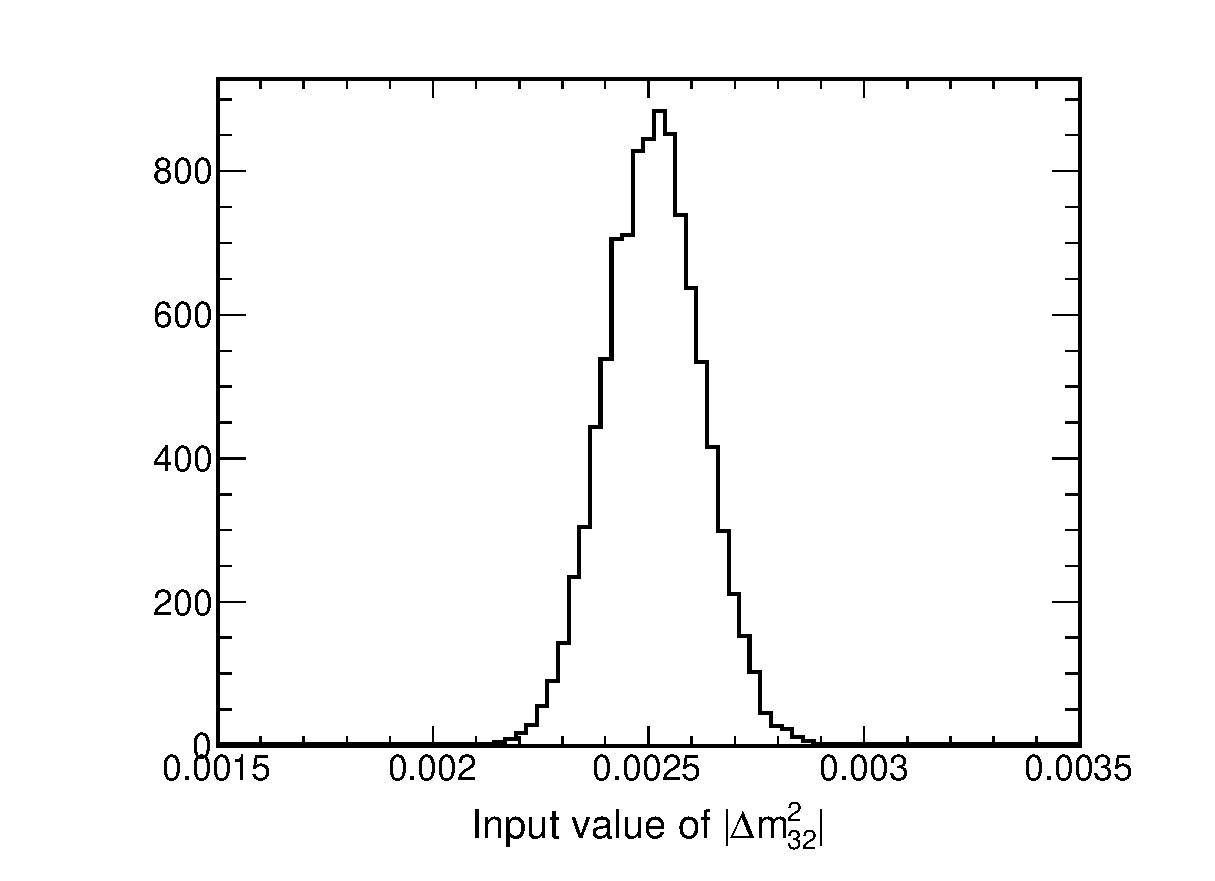
\includegraphics[width=30pc]{./images/fc_surface/input_dm32sq_for_mixing23_0point55}
    \caption {
     True input values of $|\Delta m_{32}^{2}|$ to the toy Monte Carlo experiments used to find the 1D critical value of $\Delta \chi^{2}$ 
     for $\sin^{2}\theta_{23}$ = 0.55. The normal mass hierarchy is assumed.
    }
    \label{fig:input_dm32sq_1DFC}
  \end{minipage}
  \vfill
  \begin{minipage}[t]{0.96\linewidth}
    \center
    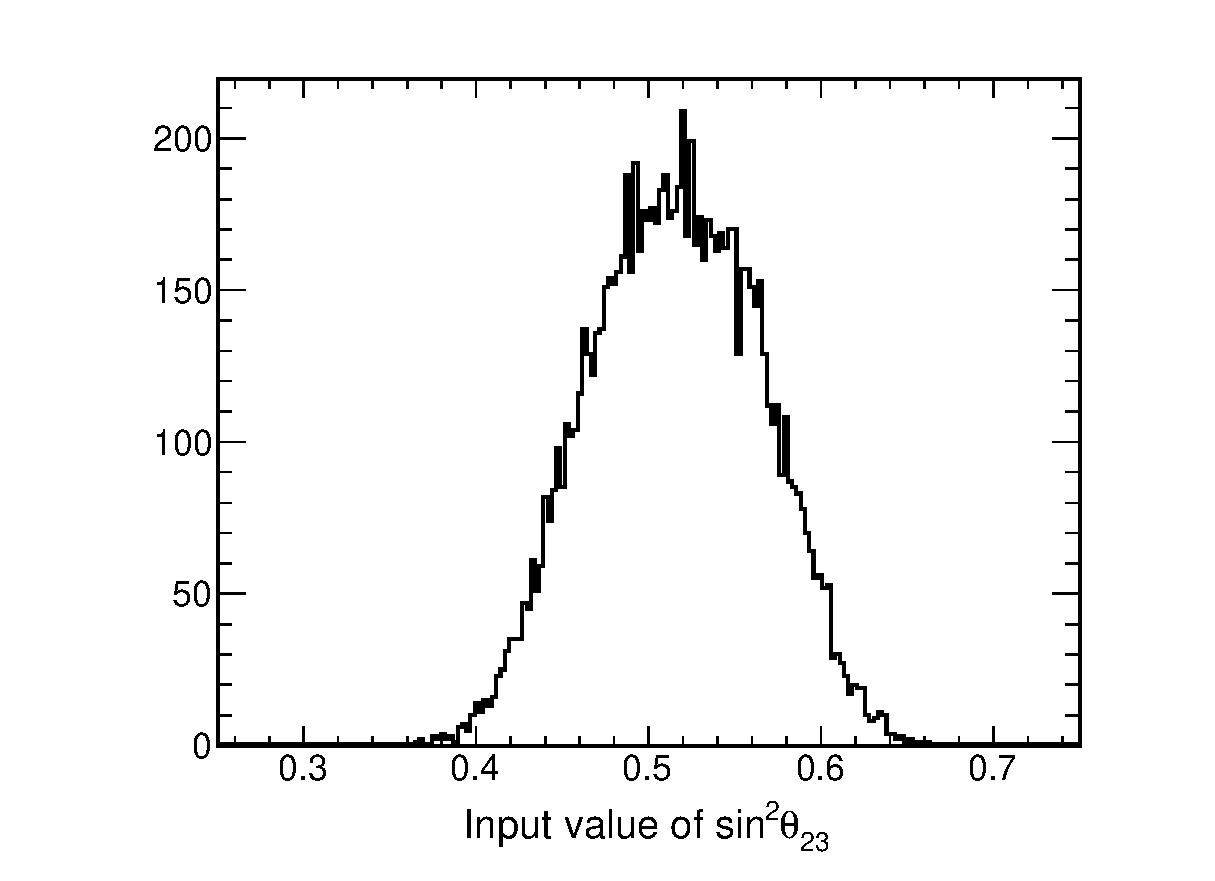
\includegraphics[width=30pc]{./images/fc_surface/input_mixing23_for_dm32sq_2point9Eminus3}
    \caption {
     True input values of $\sin^{2}\theta_{23}$ to the toy Monte Carlo experiments used to find the 1D critical value of $\Delta \chi^{2}$
     for $|\Delta m_{32}^{2}|$ = 2.9$\times$10$^{-3}$ eV$^{2}$/c$^{4}$. The normal mass hierarchy is assumed.
    }
    \label{fig:input_mixing23_1DFC}
  \end{minipage}
\end{figure*}
